Pierworodnym synem Edwarda i Eufemii Świerczyńskich był \textbf{Józef, który przyszedł na świat 14 marca 1908 r. w Łagiewnikach Wielkich}.

\begin{figure}[!h]
\begin{center}
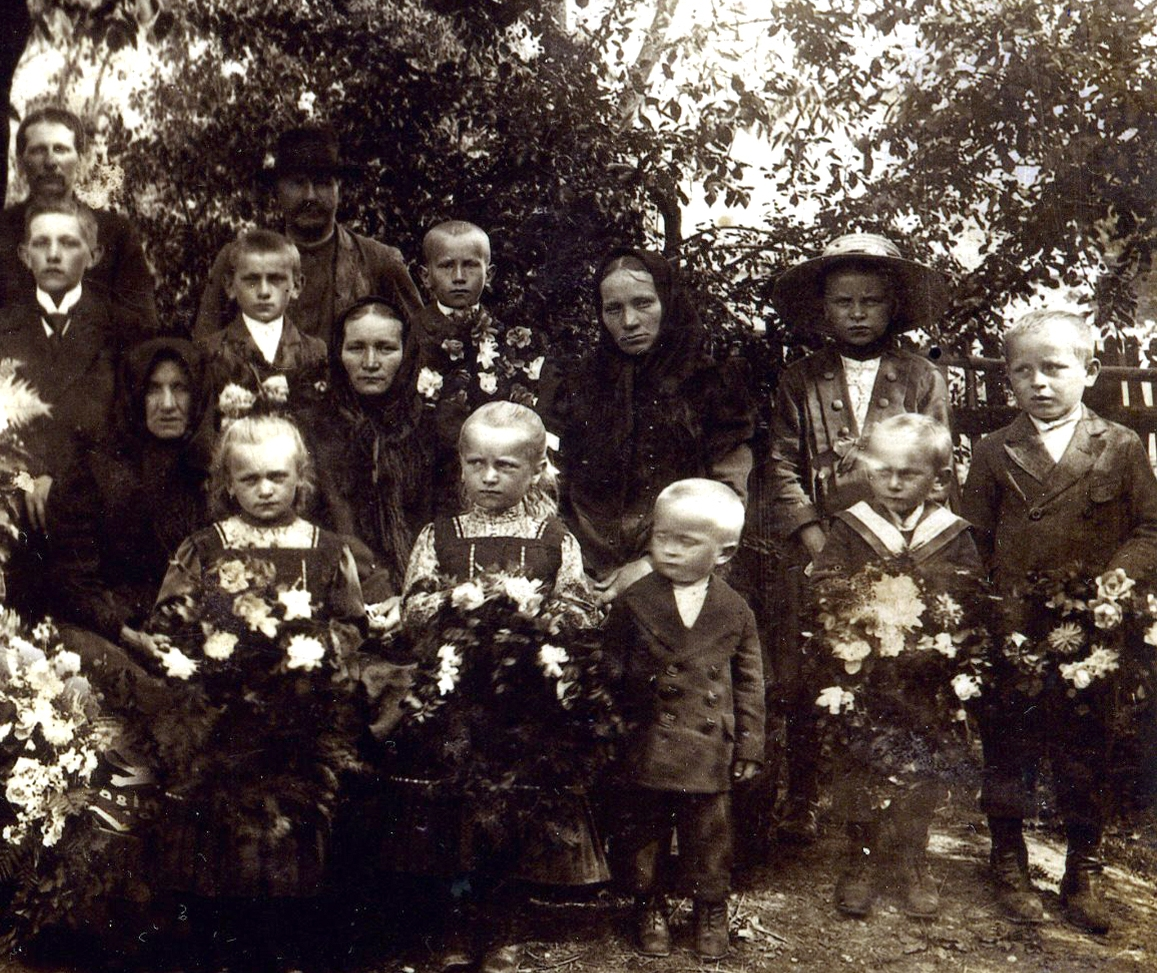
\includegraphics[width=0.5\textwidth]{photo/eufemia_swierczynska_z_dziecmi.jpg}
\caption[Eufemia Świerczyńska z dziećmi podczas pogrzebu jej ojca Jakuba Grabińskiego w 1916 r.]{Eufemia Świerczyńska z dziećmi podczas pogrzebu jej ojca Jakuba Grabińskiego w 1916 r. Przed nią stoi mały Wiktor, za nią z prawej stoi Józef Świerczyński.}
\label{rys:eufemia_swierczynska_z_dziecmi}
\end{center}
\end{figure}

Wykształcił się na geodetę i zarabiał niemałe pieniądze, których sporą część rozmienił na alkohol. \textbf{Ożenił się w Tarnowskich Górach 7 czerwca 1930~r.  ze starszą od siebie Ludwiką z domu Jabłońską, panną z Męcina pod Nowym Sączem, córką Jakuba i Marcjanny z domu Galas urodzoną 1 lipca 1905~r.} Była ona kucharką u właścicieli dworu w Łagiewnikach Wielkich.

\begin{figure}[!h]
\begin{center}
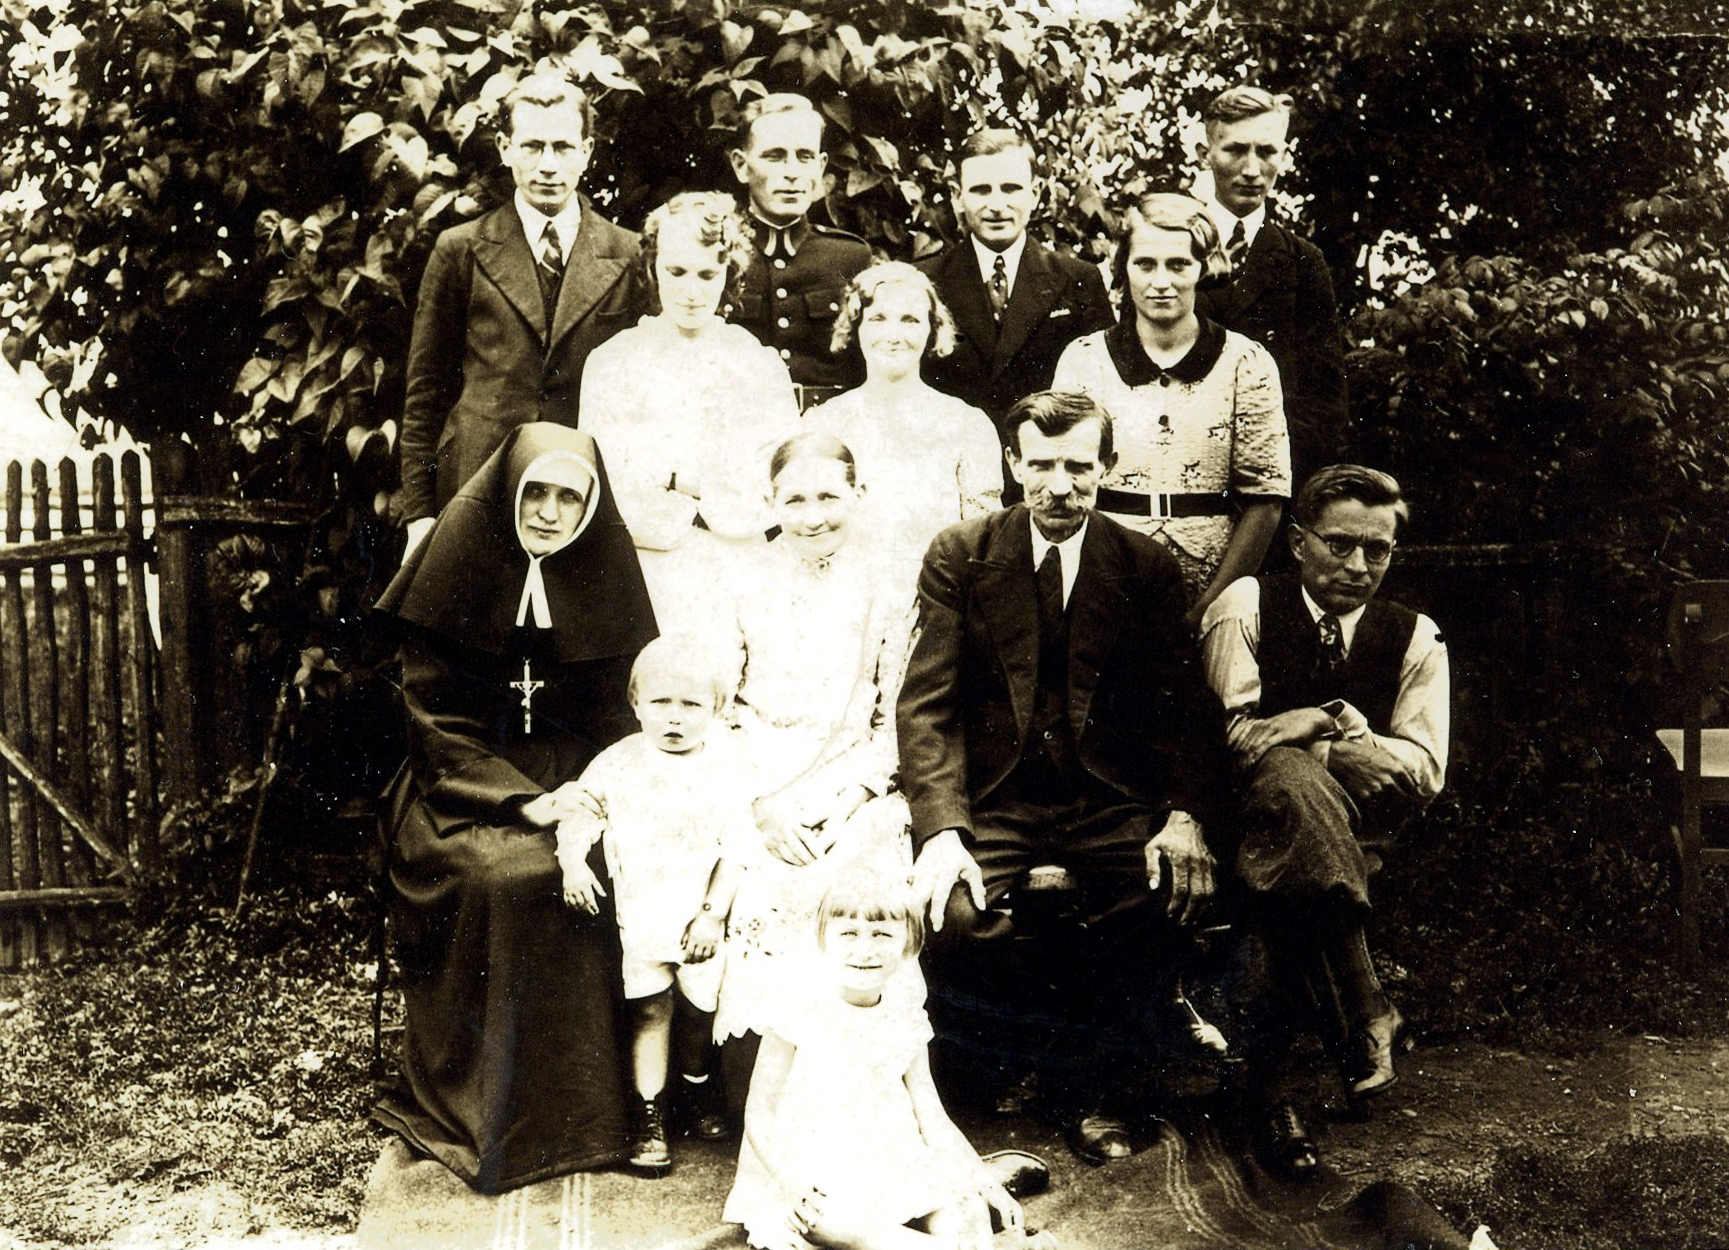
\includegraphics[width=0.7\textwidth]{photo/jozef_ludwika_swierczynscy_z_dziecmi.jpg}
\caption[Józef i Ludwika Świerczyńscy z dziećmi]{Józef i Ludwika Świerczyńscy z dziećmi. Na zdj.przed siedzącymi od lewej s. Aurelią Świerczyńską, jej matką Eufemią i ojcem Edwardem Świerczyńskim oraz Wiktorem Świerczyńskim stoi malutki Wirguś Świerczyński i siedzi przed nim Ela - jego siostra. Za nimi stoją od lewej: Józef Świerczyński, Irena Lehman, Karol Świerczyński, Ludwika Świerczyńska (żona Józefa) Antoni lehman (mąż Ireny), Róża Świerczyńska i jej brat Benedykt, wasz Dziadek.}
\label{rys:jozef_ludwika_swierczynscy_z_dziecmi}
\end{center}
\end{figure}

Ma z nią dwoje dzieci: \textbf{Elżbietę, która przyszła na świat 30 października 1930~r. w Lublińcu oraz Wirgiliusza urodzonego tamże 23 czerwca 1935~r.}.

\begin{figure}[!h]
\begin{center}
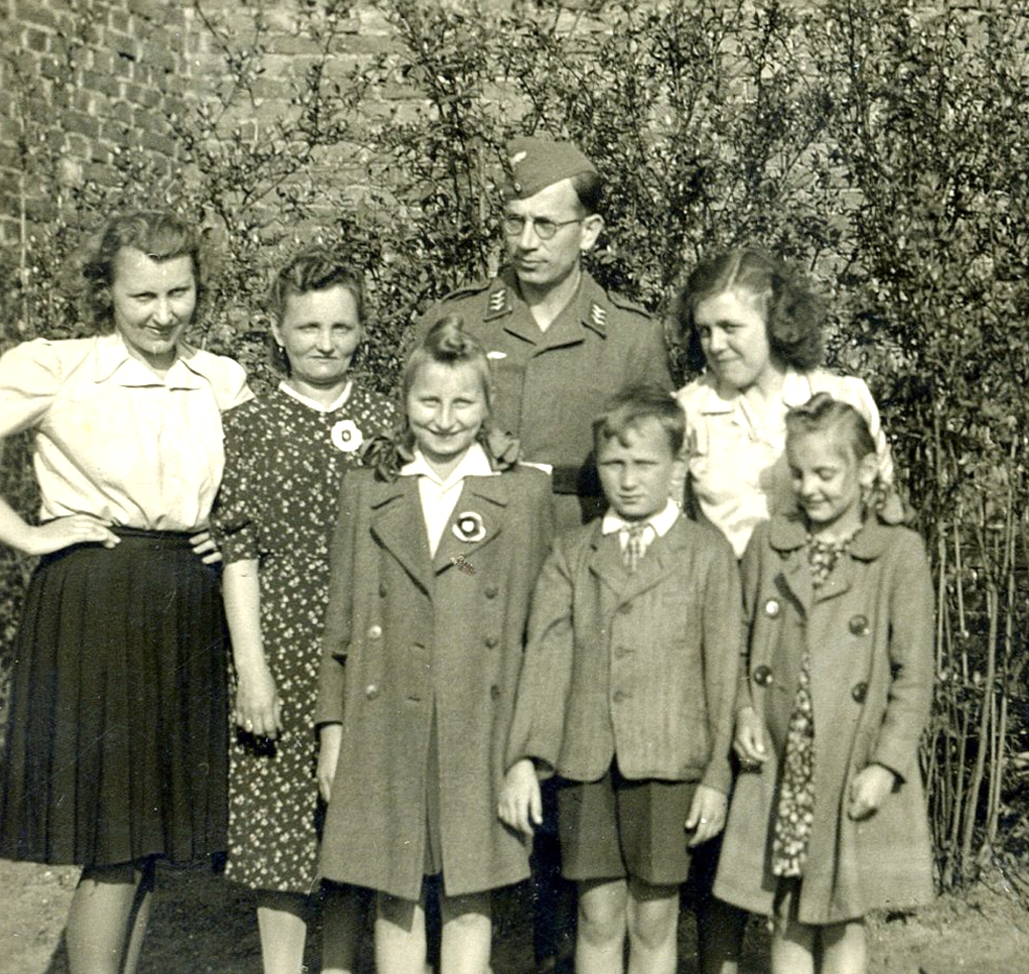
\includegraphics[width=0.5\textwidth]{photo/jozef_swierczynski.jpg}
\caption[Rodzina Józefa Świerczyńskiego]{Rodzina Józefa Świerczyńskiego, na zdj. od lewej stoją: Eugenia Jabłońska (siostra Ludwiki), Ludwika Świerczyńska, przed nią stoi jej córka Elżbieta, za nią stoi jej ojciec - Józef Świerczyński w mundurze Wehrmachtu, przed nim jego syn Wirgiliusz i NN.}
\label{rys:jozef_swierczynski.jpg}
\end{center}
\end{figure}

Stryj Józef najpierw pracował w Urzędzie Gminy w Łagiewnikach Wielkich, więc był przy rodzicach, a potem zamieszkał w Lublińcu u Lizurka na poddaszu, a następnie od 1934 r. przy ul. Opolskiej -- wówczas nr 6 (dziś 14) w domu moich dziadków -- Tomasza i Zofii Wilczków. W grudniu 1938~r. przeprowadzili się do Katowic Piotrowic. Przed tragicznym wrześniem 1939 r. mieszkali już w Katowicach Ligocie, przy ul. Gajowej 3, gdzie do dziś mieszka jego córka Elżbieta -- po mężu Adamska -- nasza najstarsza kuzynka.

Tak o stryju Józefie wspomina wasz Dziadek Benedykt: \textit{Siedmioro nas było. Troje starszych, zawsze, jak pamięć sięga, dużych, dorosłych, troje takich całkiem małych i jeden taki średni, nieszczęśliwy, bo choroba straszna nie pozwoliła rosnąć, jak tym starszym. My, młoda trójka, dopędzała go, a on stał w miejscu. Najstarszym był Józef, którego zapamiętałem jako dużego pana, który pod nieobecność rodziców próbował wodzirejować w domu. To zdarzało się bardzo rzadko, bo w domu bywał od wieczora do rana. Za dnia był albo gminnym sekretarzem albo urzędnikiem w mieście. Wracał wieczorem, czasem dość późno, zasługując na dość częste reprymendy ojca lub mamy, a rano nie można go było dobudzić.}

Stryj w czasie wojny odbywał służbę wojskową w Wehrmachcie w Magdeburgu, gdzie był do czasu, gdy Amerykanie zajęli to miasto, zaś po odbyciu służby w wojsku polskim w Szkocji zamieszkał w Edynburgu, skąd wrócił do Polski dopiero w czerwcu 1948 r. \textbf{Stryjenka Ludwika zmarła na raka 18 marca 1963~r.} i została pochowana na cmentarzu w Ligocie.

\begin{figure}[!h]
\begin{center}
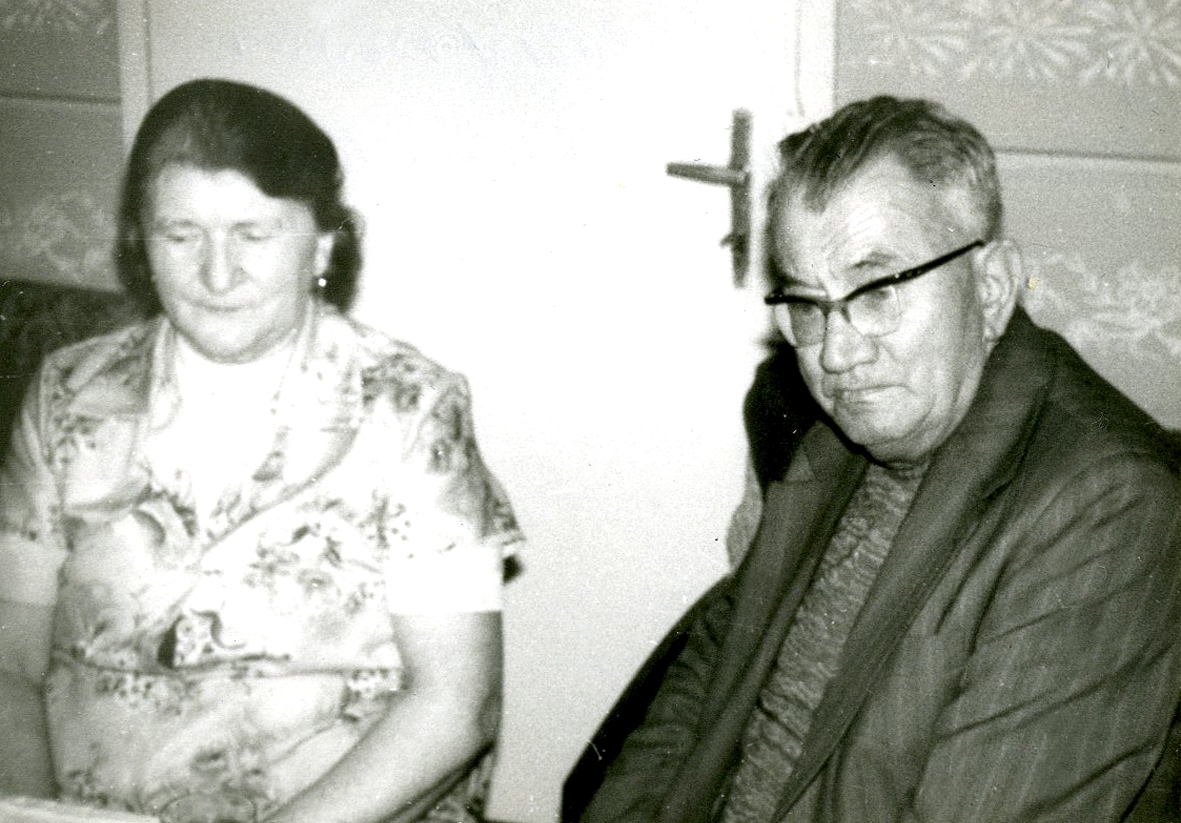
\includegraphics[width=0.55\textwidth]{photo/jozef_maria_swierczynscy.jpg}
\caption{Na zdj. Maria Goldman i Józef Świerczyński}
\label{rys:jozef_maria_swierczynscy}
\end{center}
\end{figure}

W dwa lata po jej śmierci \textbf{stryj Józef 1 czerwca 1965 r. pojął za żonę w Żernicy koło Gliwic Marię Goldman} i zamieszkał u niej. Poznał ją w firmie geodezyjnej w Gliwicach, gdzie pracował. \textbf{Zmarł w Żernicy 20 października 1985 r.}, gdzie  został pochowany. \textbf{Maria Goldmann zmarła w Żernicy 16 kwietnia 1994~r.}

Nasza najstarsza kuzynka naukę w szkole podstawowej rozpoczęła już w Katowicach, gdzie też ukończyła Technikum Krawieckie. \textbf{Elżbieta Świerczyńska zawarła ślub kościelny z Bolesławem Pudraszem, z którym się rozwiodła w Urzędzie Stanu Cywilnego. Natomiast w kwietniu 1953 r. zawarła z Tadeuszem Adamskim ur. 15 kwietnia 1924 r. w Przyłęku koło Jędrzejowa związek cywilny}, z którym nie doczekała się potomstwa, więc adoptowali oni dziewczynkę z domu dziecka -- \textbf{Jolantę urodzoną 9 stycznia 1973 r. w Katowicach}. 

\begin{figure}[!h]
\begin{center}
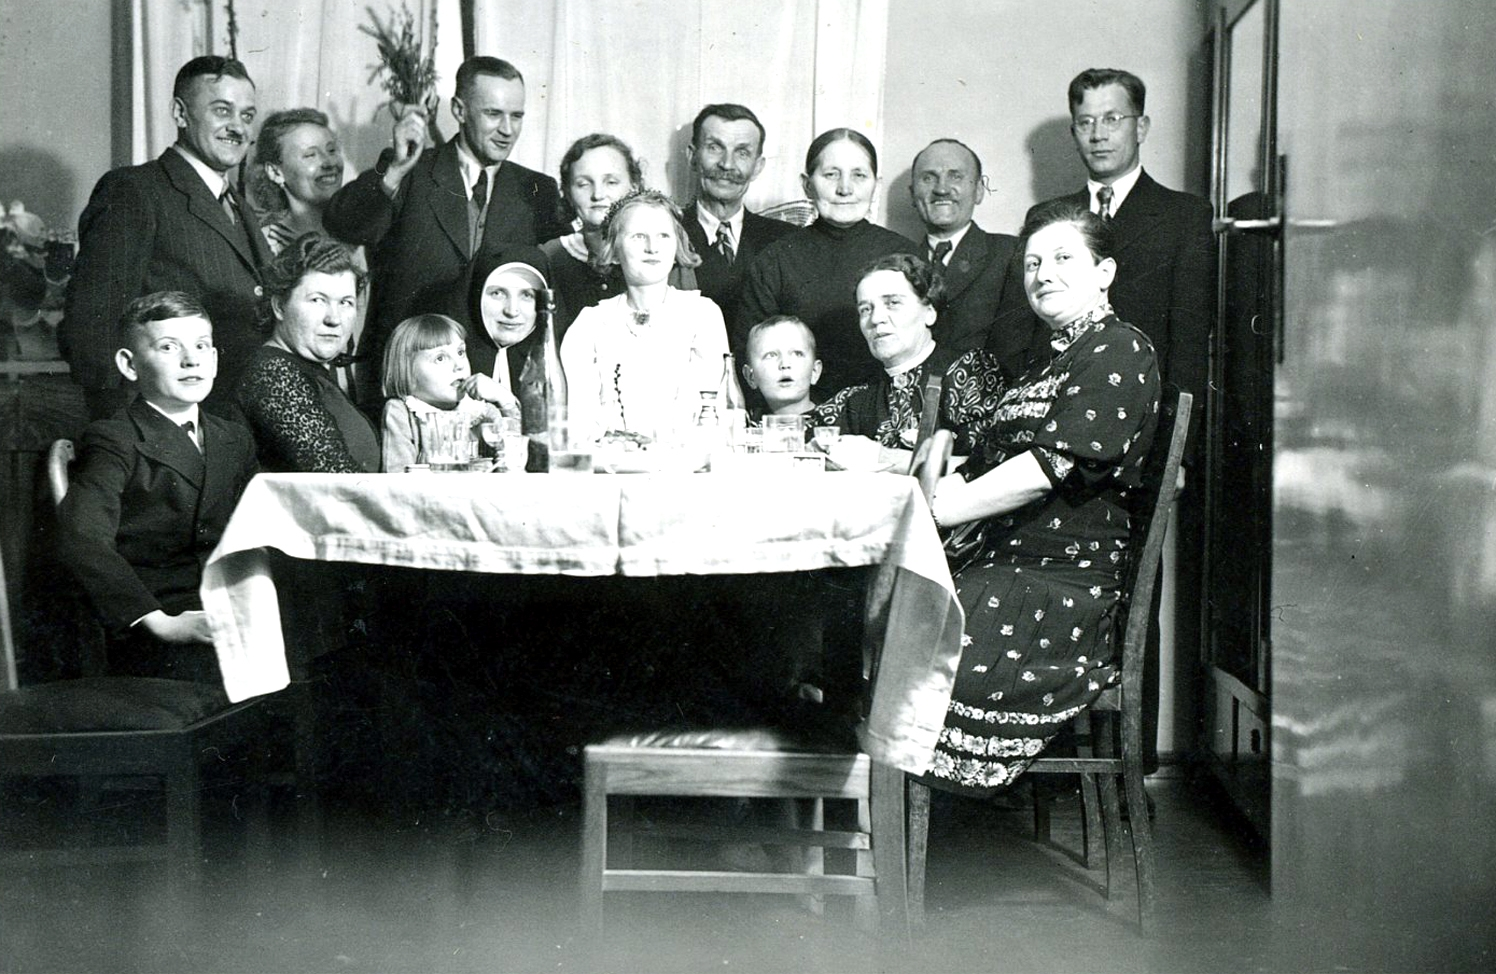
\includegraphics[width=0.7\textwidth]{photo/elzbieta_swierczynska_1.jpg}
\caption[Elżbieta Świerczyńska u I Komunii św.]{Elżbieta Świerczyńska u I Komunii św., na zdj. Ela stoi przy stole, obok niej siedzi stryjenka Aurelia Świerczyńska, z tyłu za nią stoi jej matka Ludwika, dziadek Edward i babcia Eufemia, przy drzwiach stoi jej ojciec Józef Świerczyński.}
\label{rys:elzbieta_swierczynska_1}
\end{center}
\end{figure}

\begin{figure}[!h]
\begin{center}
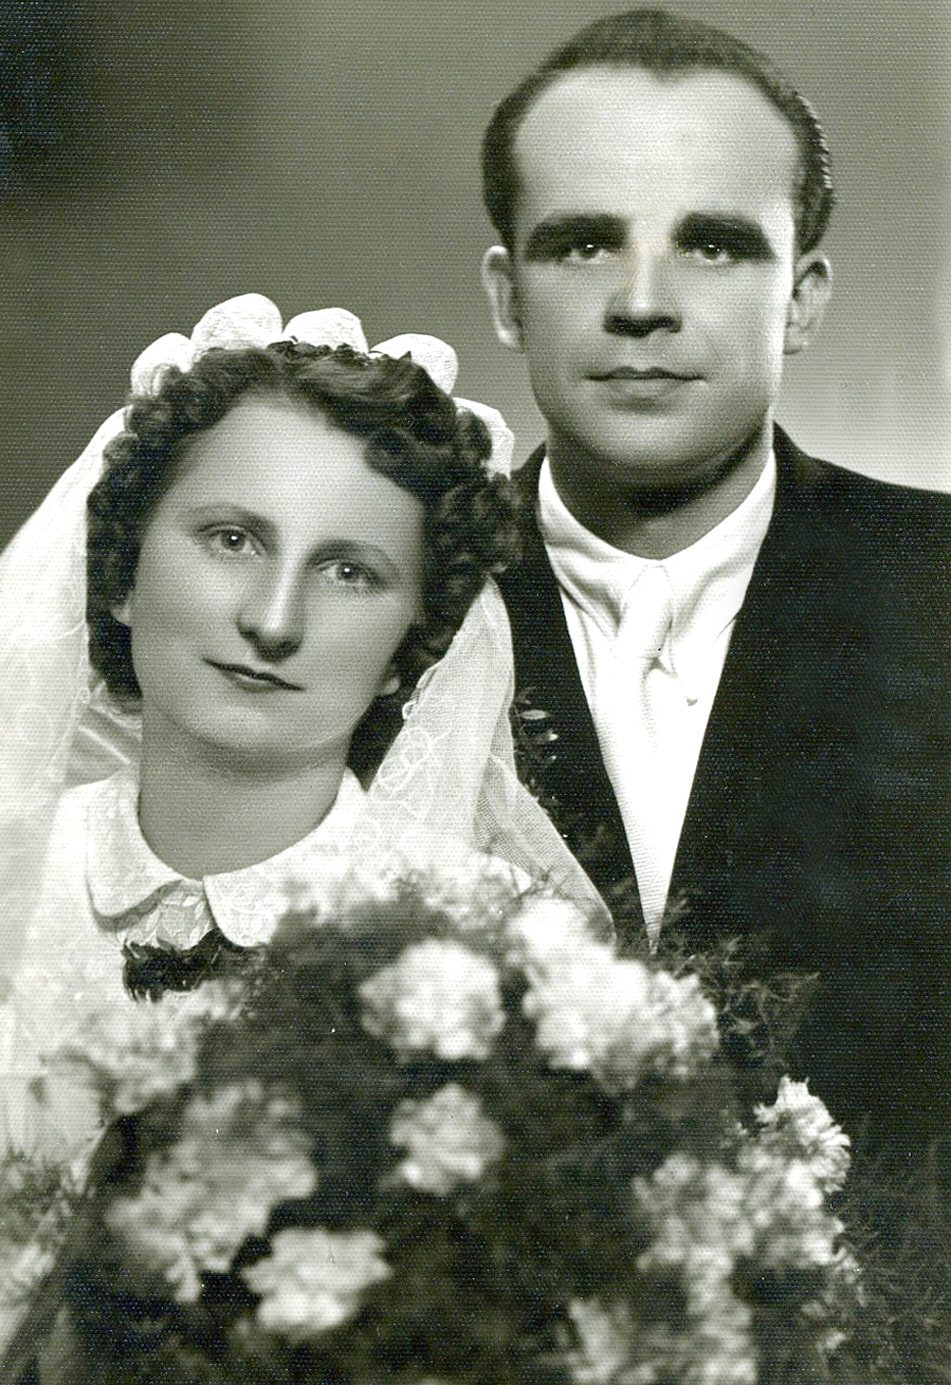
\includegraphics[width=0.3\textwidth]{photo/elzbieta_tadeusz_adamscy.jpg}
\caption{Zdjęcie ślubne Elżbiety Świerczyńskiej i Tadeusza Adamskiego}
\label{rys:elzbieta_tadeusz_adamscy}
\end{center}
\end{figure}

Jola ukończywszy naukę w Liceum Medycznym w Katowicach wyszła najpierw za Leszka Niewęgłowskiego, z którym się wkrótce rozeszła. \textbf{We wrześniu 2006 r. wyszła za Mariusza Waligórę ur. 19 sierpnia 1973 r. w Czeladzi}, który jako kierowca -- zaopatrzeniowiec utrzymuje swoją rodzinę. \textbf{Urodziła im się 26 maja 2007 r. w Katowicach córeczka -- Wiktoria.}
Tak oto Elżbieta w 77 roku życia została babcią i ofiarnie realizuje się w swym nowym powołaniu.

\begin{figure}[!h]
\begin{center}
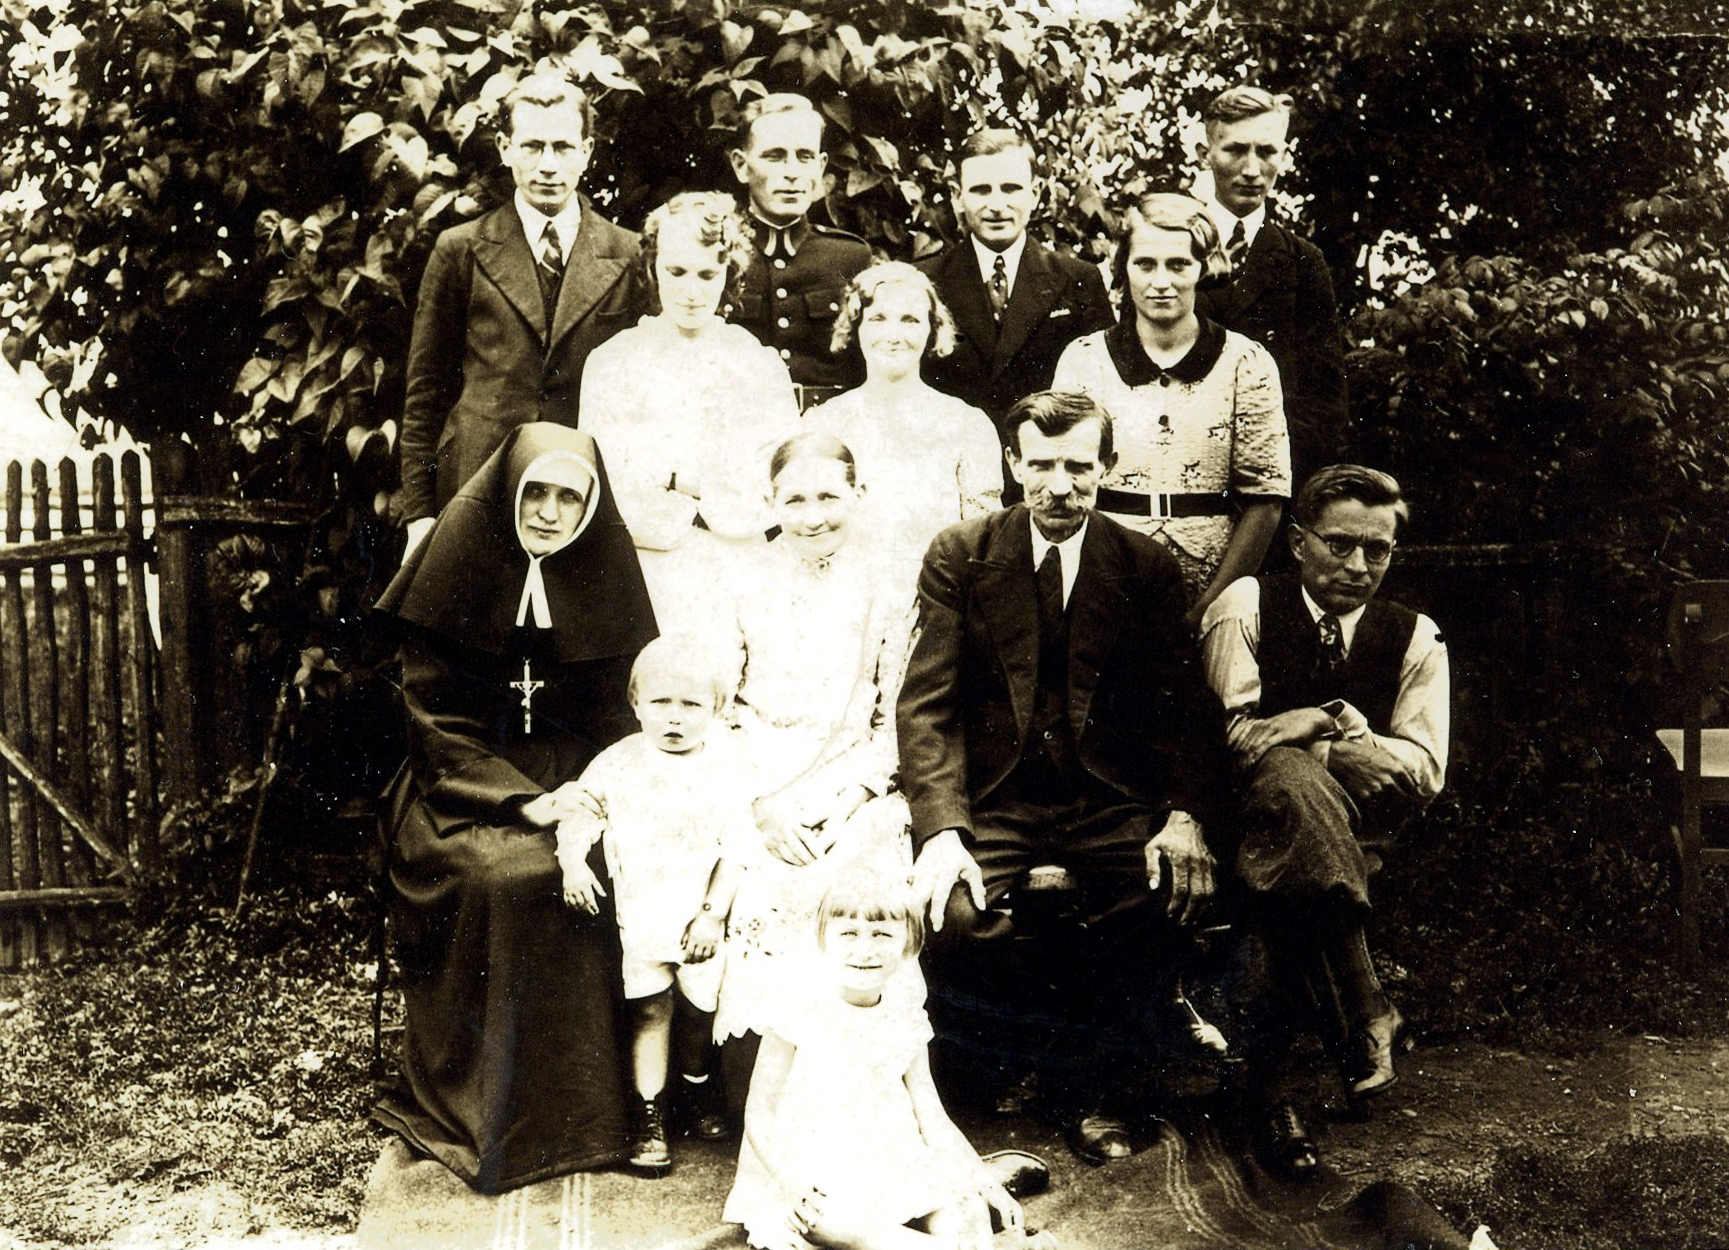
\includegraphics[width=0.6\textwidth]{photo/wirgiliusz_swierczynski_1.jpg}
\caption{Wirgiliusz Świerczyński -- trzymany za rączkę przez siostrę Aurelię}
\label{rys:wirgiliusz_swierczynski_1}
\end{center}
\end{figure}

Brat Elżbiety -- \textbf{Wirgiliusz urodzony 23 czerwca 1935 r. w Lublińcu}, ukończył Technikum Elektryczne w Katowicach i po odbyciu służby wojskowej większość życia przepracował w Elektrowniach: w Halembie 12 lat oraz do emerytury w Rybniku. Mieszka w tym mieście w bloku przy ul. Chalotta 6/9. Pracował też trzy lata na kontrakcie w Turcji przy budowie elektrowni w południowo zachodnim ,,rogu'' Azji Mniejszej oblewanej tam falami Morza Egejskiego i Śródziemnego. Zwiedził dzięki temu Efez i miejsca związane ze św. Janem Ewangelistą, z Matką Bożą i Jej Wniebowzięciem. \textbf{Ożenił się 12 czerwca 1955 r. w Borowej Wsi koło Mikołowa z uroczą Urszulą Drygalską, córką Jana i Teresy z domu Hartwig - ur. 12 czerwca 1933 r. w Skarlinie na Pomorzu.}

\begin{figure}[!h]
\begin{center}
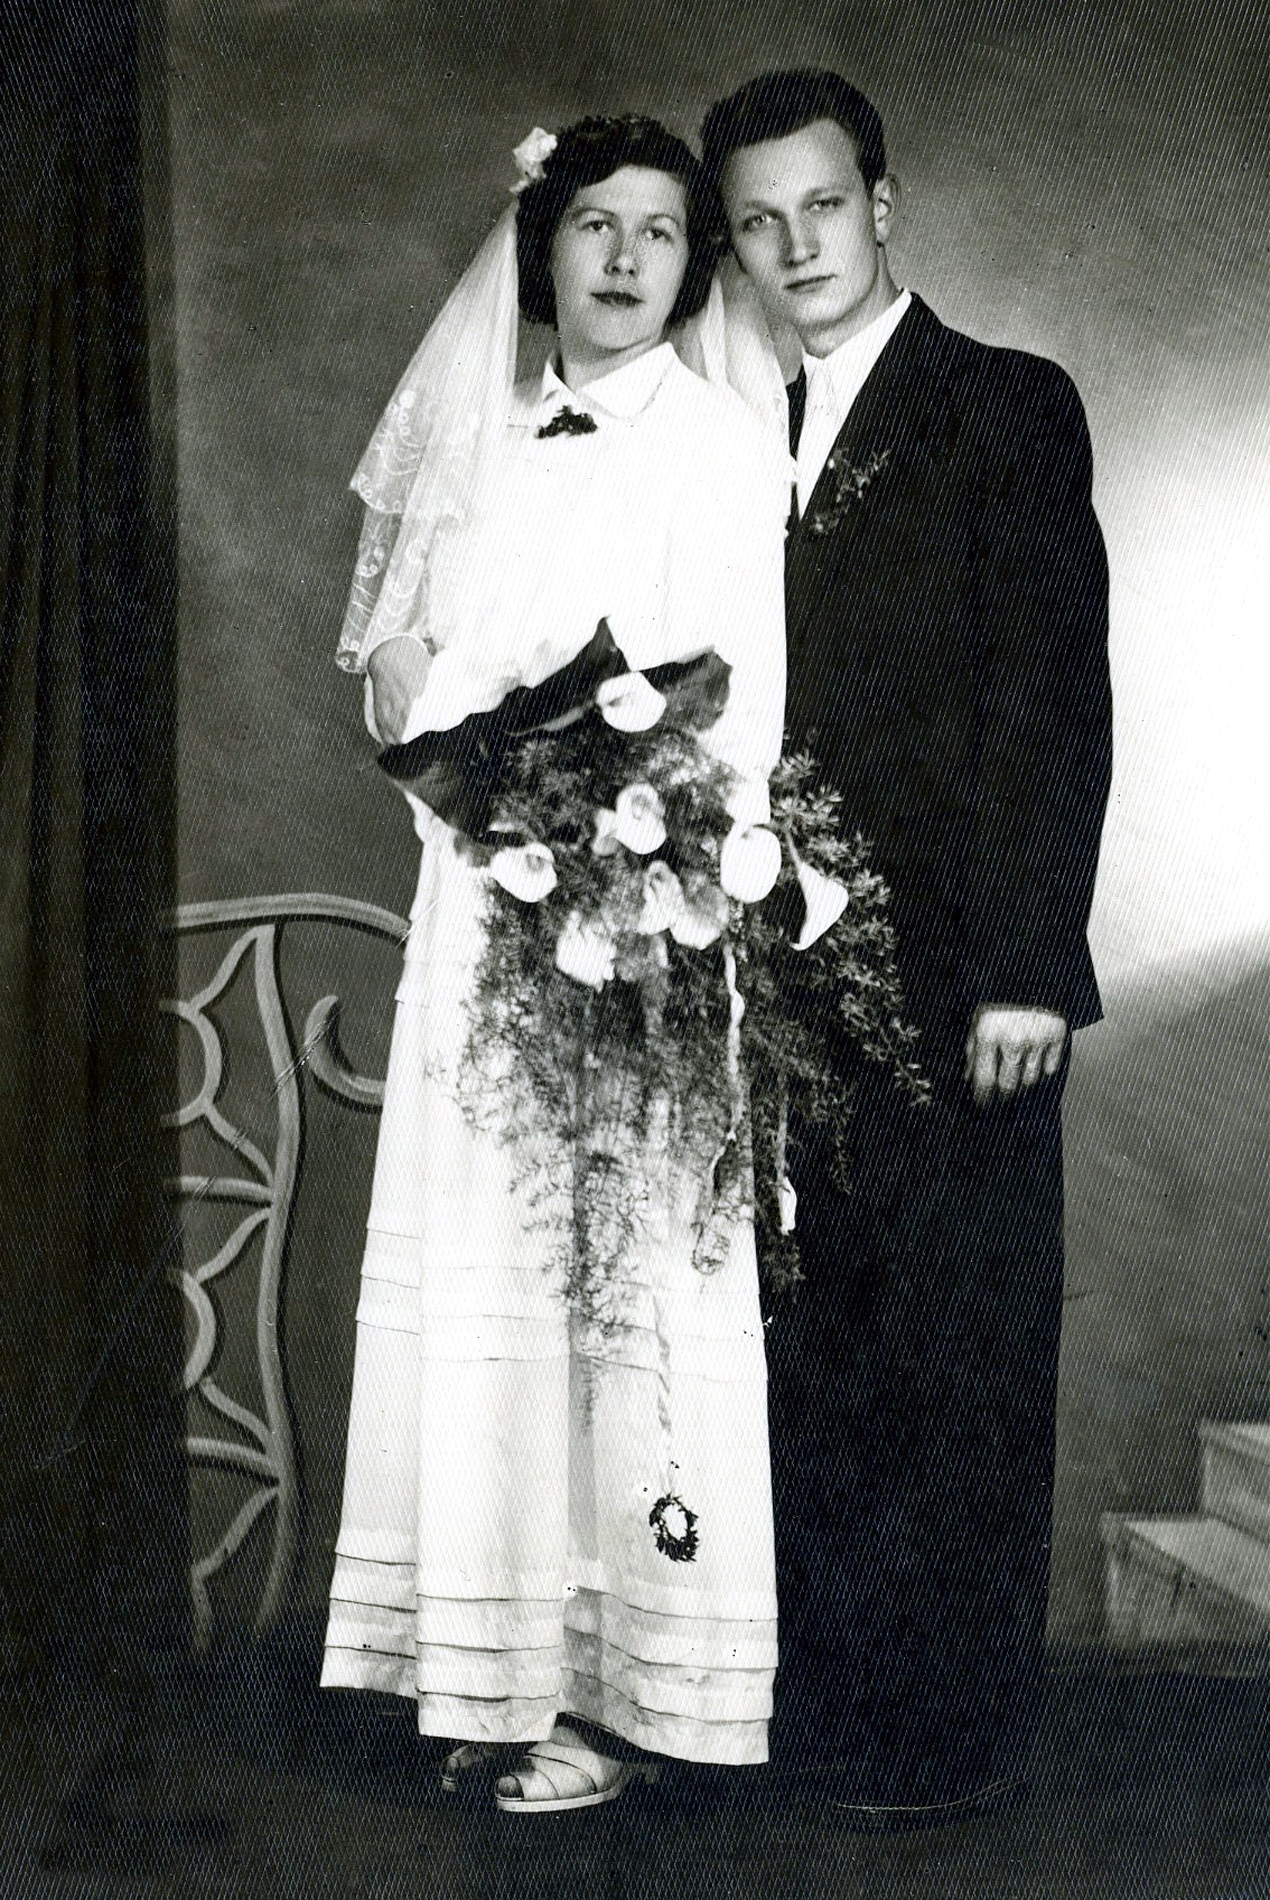
\includegraphics[width=0.3\textwidth]{photo/wirgiliusz_urszula_swierczynscy.jpg}
\caption{Zdjęcie ślubne  Urszuli Drygalskiej i Wirgiliusza Świerczyńskiego}
\label{rys:wirgiliusz_urszula_swierczynscy}
\end{center}
\end{figure}

\textbf{Ich jedyna córka - Ewa Świerczyńska przyszła na świat 22 października 1955 r. w Katowicach} i po ukończeniu Technikum Ekonomicznego w Rybniku \textbf{wyszła dnia 26 grudnia 1976 r. w Rybniku za Władysława Rosińskiego urodzonego 15 marca 1952 r. w Piotrkowie Kujawskim}.

\begin{figure}[!h]
\begin{center}
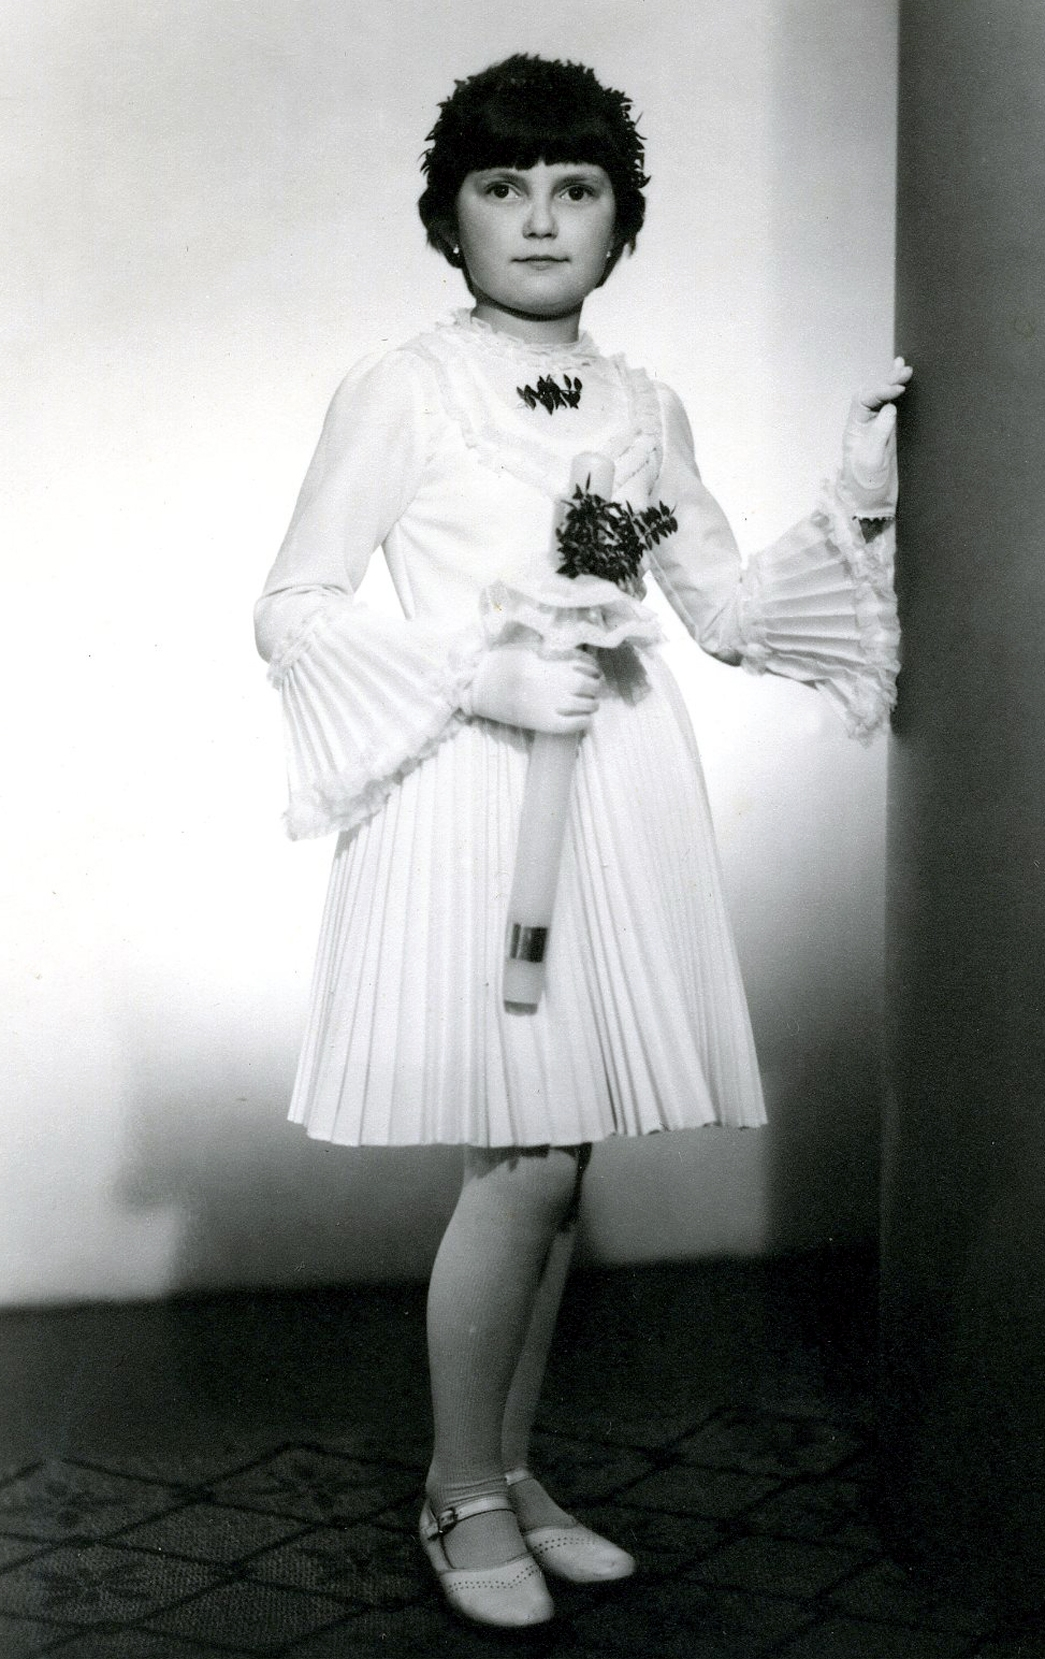
\includegraphics[width=0.3\textwidth]{photo/ewa_swierczynska.jpg}
\caption{Ewa Świerczyńska u I Komunii św.}
\label{rys:ewa_swierczynska}
\end{center}
\end{figure}

\begin{figure}[!h]
\begin{center}
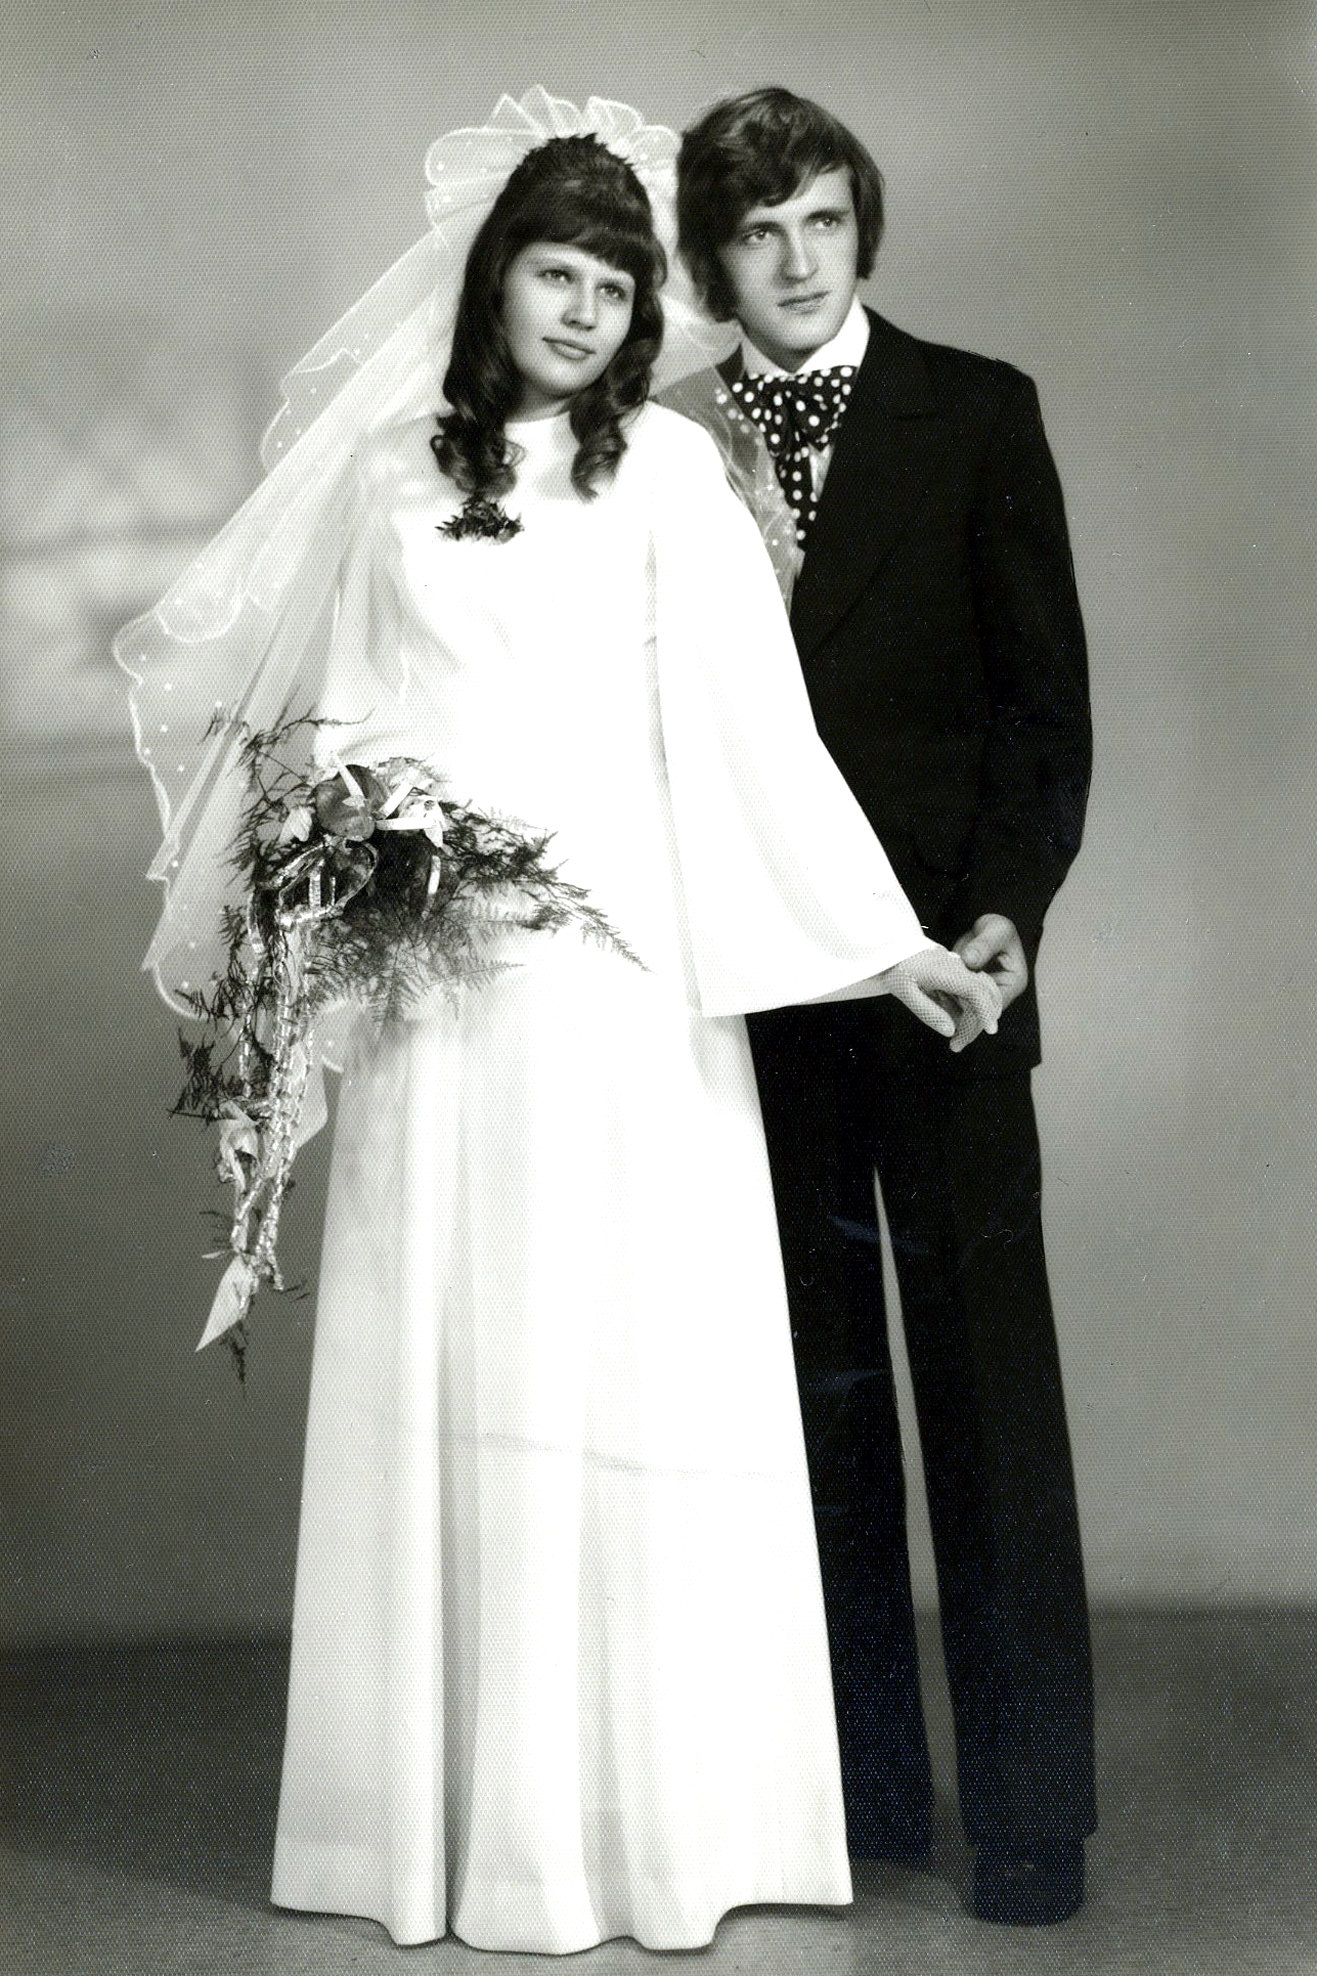
\includegraphics[width=0.35\textwidth]{photo/ewa_wladyslaw_rosinscy_slub}
\caption{Zdjęcie ślubne Ewy Świerczyńskiej i Władysława Rosińskiego}
\label{rys:ewa_wladyslaw_rosinscy_slub}
\end{center}
\end{figure}

Władek ukończył Technikum Energetyczne w Rybniku i pracuje w tamtejszej elektrowni. Wybudowali oni sobie dom w Zebrzydowicach pod Rybnikiem (dziś ul. Równa 5 w Rybniku), w czym im pomógł Wirgiliusz. Z ich związku \textbf{przyszedł na świat 22 października 1979 r. w Katowicach Marek Rosiński} pod czujnym okiem stryjenki Ireny.

\begin{figure}[!h]
\begin{center}
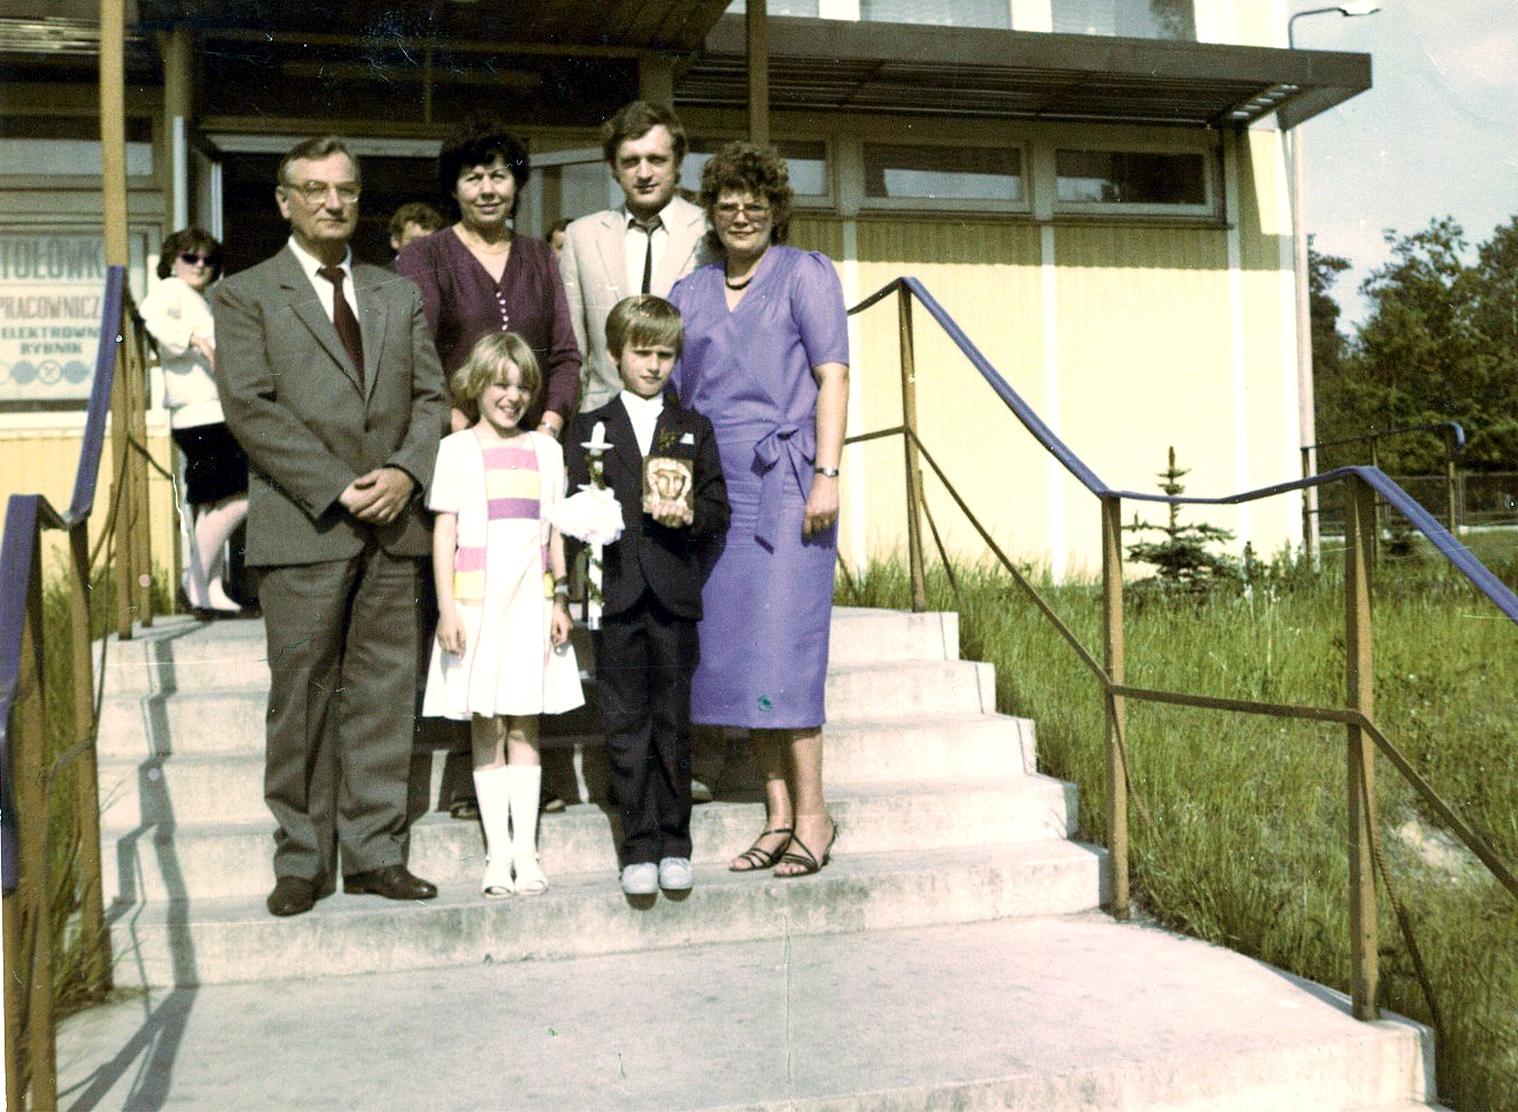
\includegraphics[width=0.6\textwidth]{photo/marek_rosinski_komunia.jpg}
\caption[Pierwsza Komunia św. Marka Rosińskiego]{Pierwsza Komunia św. Marka Rosińskiego. Na zdj. od lewej Wirgiliusz Świerczyński z żoną Urszulą, Władysław i Ewa Rosińscy. Przed nimi stoi Marek Rosiński ze świecą.}
\label{rys:marek_rosinski_komunia}
\end{center}
\end{figure}

Ukończył on Technikum Budowlane i pracuje w firmie ,,Panat'' jako koordynator ds. kurierów. Ożenił się 2 października 2005 r. w Gdowie koło Chałupek z Anną Orłowską urodzoną 16 kwietnia1983 r. w Rybniku.

Jest ona absolwentką Liceum Ogólnokształcącego w Rybniku, a ponieważ zna trzy języki obce pracuje w międzynarodowej firmie transportowej. Mieszkają przy rodzicach w Rybniku przy ul Równej. Na razie nie mają dzieci.